%-----------------------------------------------%
%             filename: skeleton.tex
%-----------------------------------------------%
\documentclass[aps,twocolumn]{revtex4}
\usepackage{graphicx}
\usepackage{ifpdf}
\ifpdf
	\usepackage[backref]{hyperref}
	%\usepackage[backref,pageanchor=true,plainpages=false, pdfpagelabels,bookmarks,bookmarksnumbered]	{hyperref}
\else
\fi

\usepackage{crs}

\begin{document} 

\title{\bf The evolution of information representation in biological networks}

\author{Cameron Ray Smith$^{1}$, Aviv Bergman$^{1,2,3}$}

\affiliation{$^1$Department of Systems and Computational Biology,\\ $^2$Dominick P. Purpura Department of Neuroscience, \\ $^3$Department of Pathology, Albert Einstein College of Medicine, 1301 Morris Park Ave, Bronx, NY 10461, USA}

\date{\today}
\begin{abstract}
Abstract text
\end{abstract}

\maketitle

\tableofcontents

\section{Hierarchy in logic}

\subsection{Russell's paradox}
A theorem due to Cantor states that given a set $X$ and a map of sets $f$ it is impossible to find a mapping $$ f: X \rightarrow 2^X $$ where $2^X$ represents the set of all subsets of $X$ also referred to as the powerset of $X$.

\subsection{A type theoretic resolution}

\subsection{Categorical type theory}
See \cite{Crole1994a}.

\section{Information representation}

\subsection{Information theory}
See \cite{Ellerman2008} and \cite{Cover2006}.

\subsection{Signaling games}
See \cite{Huttegger2007}.

\subsection{Domain theory}
See \cite{Abramsky}, \cite{Abramsky1995}.

\section{Biological information}
\subsection{Niche construction and multilevel selection}
The concept of selection is foundational to evolutionary theory. More recently, a concept referred to as niche construction that we consider to be complementary to selection, in a sense to be made precise, has been introduced \cite{Odling-Smee2003,Krakauer2009}. An organism experiences a situation similar to that represented in diagram \ref{eq:intrep}. 

\begin{equation} \label{eq:intrep}
\begin{tikzcd}[column sep=huge,row sep=huge,baseline=(current bounding box.center)]
\mathcal{D}
  \arrow[loop left]{}[name=fg]{F \circ G}
  \rar[start anchor=30, end anchor=151]{G}
  \arrow{d}[swap,name=h]{H} & 
\mathcal{J}\lar[start anchor=196, end anchor=-14]{F} \\
\mathcal{C}
\arrow[shorten >=3pt,Rightarrow,to path={(fg.290) to[out=-90,in=180] node[xshift=-3.5mm] {$\eta$} (h)}]{}
\end{tikzcd}
\end{equation} 

The molecular interaction network that underlies an arbitrary type of organism is represented by a category $\mathcal{D}$ and the environment is represented by a category $\mathcal{C}$. Due to the dependence of selection on the environment, those organisms capable of survival are those that most closely approximate a natural transformation $\eta:F \circ G \Rightarrow H$. Why might this be the case?

To answer this question requires consideration of the necessity of the category $\mathcal{J}$ in this conceptual framework. From the perspective of any organism, we can roughly think of $\mathcal{D}$ as ''internal'' and $\mathcal{C}$ as ''external'' in a sense that can be likened but not yet clearly identified with ''known'' and ''unknown'' respectively. The selection process can be thought of as requiring the organism to establish a representation of properties of $\mathcal{C}$ so as to enable its existence to remain complementary, and thus stable, relative to its environment. The molecular network underlying the various biochemical functions of the organism has no direct access to the processes that determine the causal structure of the environment. In this case we consider the organism to have direct access only to the structure contained in $\mathcal{D}$, but nevertheless being implicitly assigned, as a result of its relationship to the environment, the seemingly impossible task of establishing the structure of $\mathcal{C}$. If $\mathcal{C}$ were internalized by the organism then relationships between $\mathcal{D}$ and $\mathcal{C}$ that preserve structure, specifically the functors labelled $H:\mathcal{D} \rightarrow \mathcal{C}$, could also be directly internalized. Since $\mathcal{C}$ is external to $\mathcal{D}$, the organism must find another way of determining the relationship between its internal structure and that which is external, even if local.

One way to address this apparently paradoxical situation is to consider the relationship between endofunctors on $\mathcal{D}$ and those like $H$. In the case of \ref{eq:intrep}, $\mathcal{J}$ is considered to be a subcategory of $\mathcal{D}$ that contains all the domains (in the sense of complete partial orders) of $\mathcal{D}$. This scenario allows functors $F:\mathcal{J} \rightarrow \mathcal{D}$ to index diagrams in $\mathcal{D}$.

See \cite{Okasha2006} for information on multilevel selection.

\subsection{The structure of molecular networks}
\subsubsection{Endo-genetics, genetics, epi-genetics, and $n$-epi-genetics}
\subsection{Hierarchical organization and evolution}
See \cite{Gould1994}, \cite{Arnold1982}.

\section*{Acknowledgements} 

CRS was supported by . 
AB was supported by .

%-----------------------------------------------%
%                   appendix
%-----------------------------------------------%
\appendix
\section{Category theory for tourists}
%\begin{figure}
%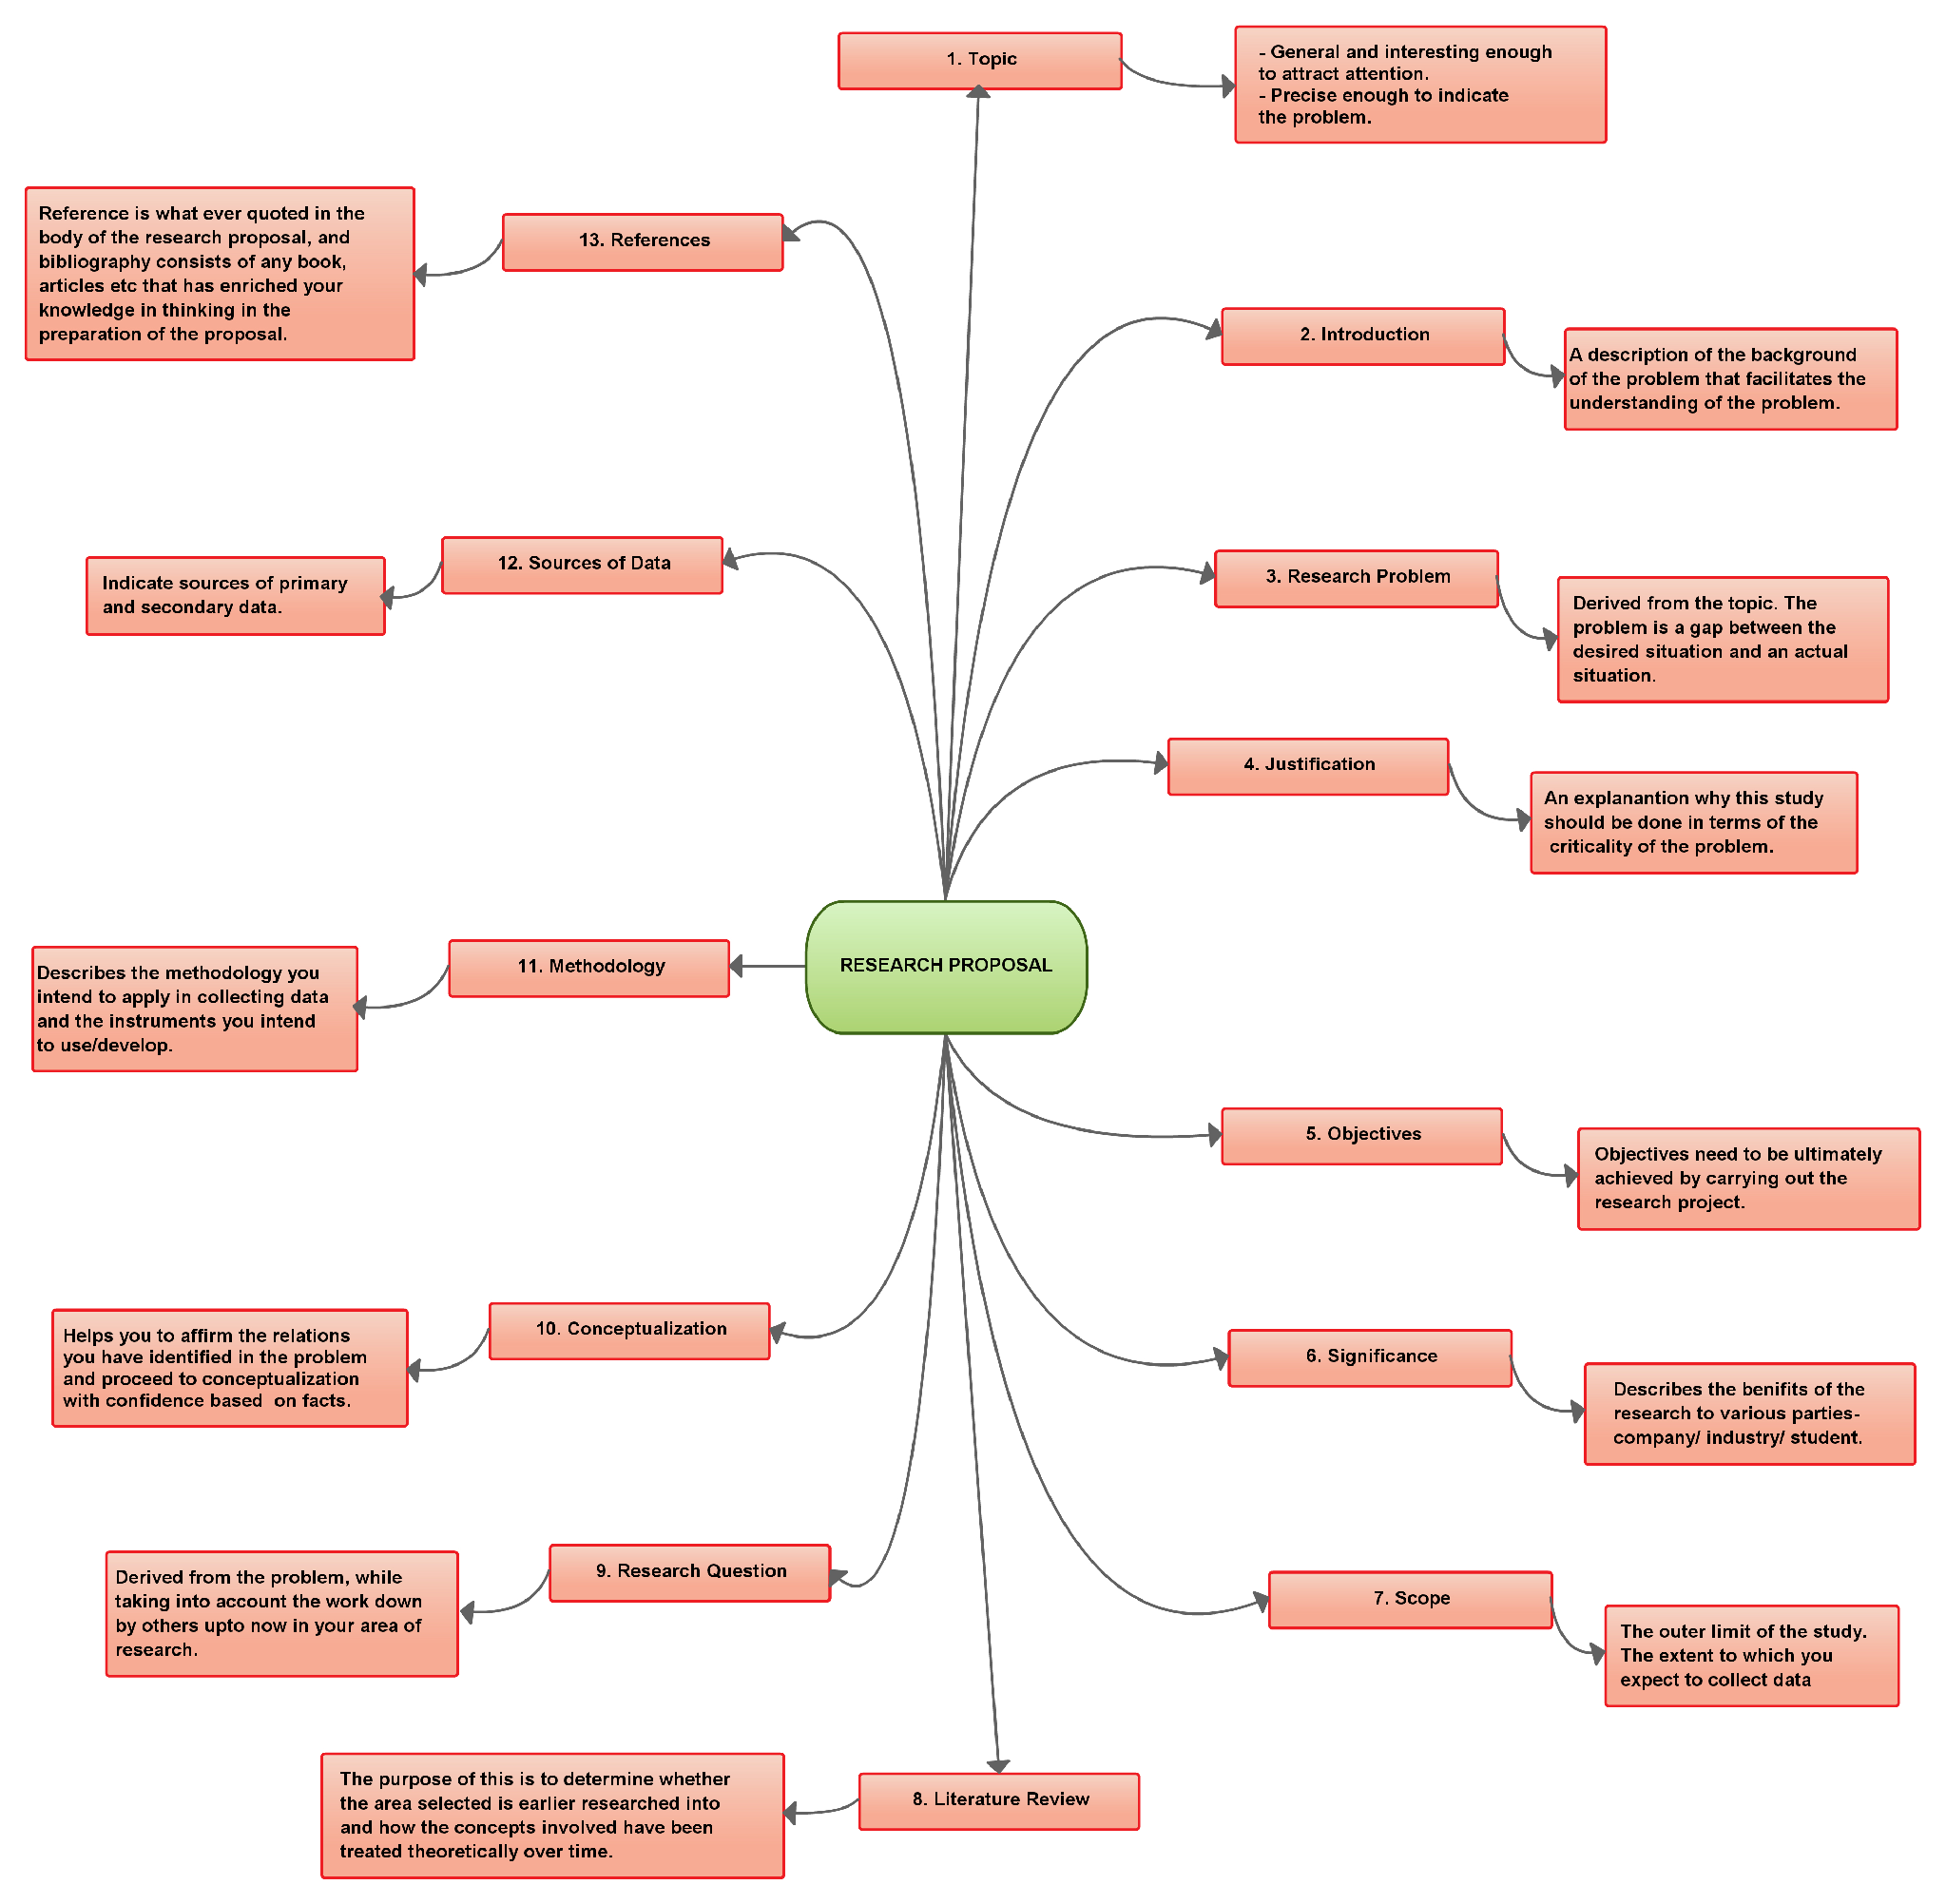
\includegraphics[scale=0.2]{fig/createlytest1.pdf}
%\caption{This is a $\implies$ creately.com diagram}
%\end{figure}
%
%\begin{center}
%\asyinclude{fig/comdiag.asy}
%\end{center}
%
%\begin{equation}\label{eq:star}
%\xymatrix{
%{\mathcal V}  \ar[r]^{S \quad\quad } \ar[d]_{\pi}
%&  \mathsf{DynSys} \ar[d]^{U}  \\
% \op{(\et{\Graph})}  \ar[r]^{\quad\mathbb{P} }
%&  \mathsf{Man} }
%\end{equation}
%
%Two related questions \cite{Gould1994} define a fundamental role for statistical
%physics in systems biology: (1). How do biomolecular systems achieve
%reliable ``device-level'' behavior when they consist of highly
%
%\begin{equation*}
%\xy
%(-18, 10)*+{\PP\lv T} ="1"; 
%(18, 10)*+{\PP\rt T} ="2";
%(-18,-10)*+{\PP\lv T'}="3";
%(18,-10)*+{\PP \rt T'}="4";
%{\ar@{->}^X "1";"2"};
%{\ar@{->}^{\PP(\sigma|_{\lv T})} "3";"1"};
%{\ar@{=}_{\PP(\sigma|_{\rt T}) = id } "4";"2"};
%{\ar@{-->}_{\Ctrl(\sigma)X} "3";"4"};
%\endxy
%\end{equation*}
%
%\begin{center}
%\begin{tikzpicture}[shorten >=1pt,->]
%  \tikzstyle{vertex}=[circle,fill=black!25,minimum size=17pt,inner sep=0pt]
%
%  \foreach \name/\x in {s/1, 2/2, 3/3, 4/4, 15/11, 
%                        16/12, 17/13, 18/14, 19/15, t/16}
%    \node[vertex] (G-\name) at (\x,0) {$\name$};
%
%  \foreach \name/\angle/\text in {P-1/234/5, P-2/162/6, 
%                                  P-3/90/7, P-4/18/8, P-5/-54/9}
%    \node[vertex,xshift=6cm,yshift=.5cm] (\name) at (\angle:1cm) {$\text$};
%
%  \foreach \name/\angle/\text in {Q-1/234/10, Q-2/162/11, 
%                                  Q-3/90/12, Q-4/18/13, Q-5/-54/14}
%    \node[vertex,xshift=9cm,yshift=.5cm] (\name) at (\angle:1cm) {$\text$};
%
%  \foreach \from/\to in {s/2,2/3,3/4,3/4,15/16,16/17,17/18,18/19,19/t}
%    \draw (G-\from) -- (G-\to);
%
%  \foreach \from/\to in {1/2,2/3,3/4,4/5,5/1,1/3,2/4,3/5,4/1,5/2}
%    { \draw (P-\from) -- (P-\to); \draw (Q-\from) -- (Q-\to); }
%
%  \draw (G-3) .. controls +(-30:2cm) and +(-150:1cm) .. (Q-1);
%  \draw (Q-5) -- (G-15);
%\end{tikzpicture}
%\end{center}
%
%
%\usetikzlibrary{matrix,arrows}
%\begin{equation}
%\begin{tikzpicture}[description/.style={fill=white,inner sep=2pt}, baseline=(current bounding box.center)]
%	\matrix (m) [matrix of math nodes, row sep=3em,
%	column sep=2.5em, text height=1.5ex, text depth=0.25ex]
%	{ A & & B \\
%	& C & \\ };
%	\path[->,font=\scriptsize]
%	(m-1-1) edge node[auto] {$ \varphi $} (m-1-3)
%	edge node[description] {$ \Psi $} (m-2-2)
%	(m-1-3) edge node[auto] {$ \Phi $} (m-2-2);
%\end{tikzpicture}
%\end{equation}

%------bibliography---%
\bibliographystyle{unsrt} 
%\bibliography{ref/HO}
\bibliography{bib/books,bib/papers}
%\bibliography{library}
%---------------------%

\end{document}